% formal/sat.tex
% mainfile: ../perfbook.tex
% SPDX-License-Identifier: CC-BY-SA-3.0

\section{SAT Solvers}
\label{sec:formal:SAT Solvers}
%
\epigraph{Live by the heuristic, die by the heuristic.}{\emph{Unknown}}

Any finite program with bounded loops and recursion can be converted
into a logic expression, which might express that program's assertions
in terms of its inputs.
Given such a logic expression, it would be quite interesting to know
whether any possible combinations of inputs could result in one of
the assertions triggering.
If the inputs are expressed as combinations of boolean variables,
this is simply SAT, also known as the satisfiability problem.
SAT solvers are heavily used in verification of hardware, which has
motivated great advances.
A world-class early 1990s SAT solver might be able to handle a logic
expression with 100 distinct boolean variables, but by the early 2010s
million-variable SAT solvers were readily
available~\cite{Kroening:2008:DPA:1391237}.

\begin{figure}
\centering
\resizebox{2in}{!}{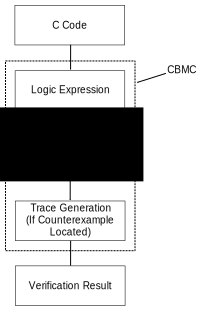
\includegraphics{formal/cbmc}}
\caption{CBMC Processing Flow}
\label{fig:formal:CBMC Processing Flow}
\end{figure}

In addition, front-end programs for SAT solvers can automatically translate
C code into logic expressions, taking assertions into account and generating
assertions for error conditions such as array-bounds errors.
One example is the C bounded model checker, or \co{cbmc}, which is
available as part of many Linux distributions.
This tool is quite easy to use, with \co{cbmc test.c} sufficing to
validate \path{test.c}, resulting in the processing flow shown in
\cref{fig:formal:CBMC Processing Flow}.
This ease of use is exceedingly important because it opens the door
to formal verification being incorporated into regression-testing
frameworks.
In contrast, the traditional tools that require non-trivial translation
to a special-purpose language are confined to design-time verification.

More recently, SAT solvers have appeared that handle parallel code.
These solvers operate by converting the input code into single static
assignment (SSA) form, then generating all permitted access orders.
This approach seems promising, but it remains to be seen how well
it works in practice.
One encouraging sign is work in 2016 applying \co{cbmc} to Linux-kernel
RCU~\cite{LihaoLiang2016VerifyTreeRCU,Liang:2018:VTB,LanceRoy2017CBMC-SRCU}.
This work used minimal configurations of RCU, and verified scenarios
using small numbers of threads, but nevertheless successfully ingested
Linux-kernel C code and produced a useful result.
The logic expressions generated from the C code had up to 90~million
variables, 450~million clauses, occupied tens of gigabytes of memory,
and required up to 80~hours of CPU time for the SAT solver to produce
the correct result.

Nevertheless, a Linux-kernel hacker might be justified in feeling skeptical
of a claim that his or her code had been automatically verified, and
such hackers would find many fellow skeptics going back
decades~\cite{DeMillo:1979:SPP:359104.359106}.
One way to productively express such skepticism is to provide bug-injected
versions of the allegedly verified code.
If the formal-verification tool finds all the injected bugs, our hacker
might gain more confidence in the tool's capabilities.
Of course, tools that find valid bugs of which the hacker was not yet aware
will likely engender even more confidence.
And this is exactly why there is a \co{git} archive with a 20-branch set
of mutations, with each branch potentially containing a bug injected
into Linux-kernel RCU~\cite{PaulEMcKenney2017VerificationChallenge6}.
Anyone with a formal-verification tool is cordially invited to try that
tool out on this set of verification challenges.

Currently, \co{cbmc} is able to find a number of injected bugs,
however, it has not yet been able to locate a bug that RCU's
maintainer was not already aware of.
Nevertheless, there is some reason to hope that SAT solvers will someday
be useful for finding concurrency bugs in parallel code.
